\begin{figure}[ht]
  \centering
  
  \begin{subfigure}[ht]{.33\linewidth}
    \centering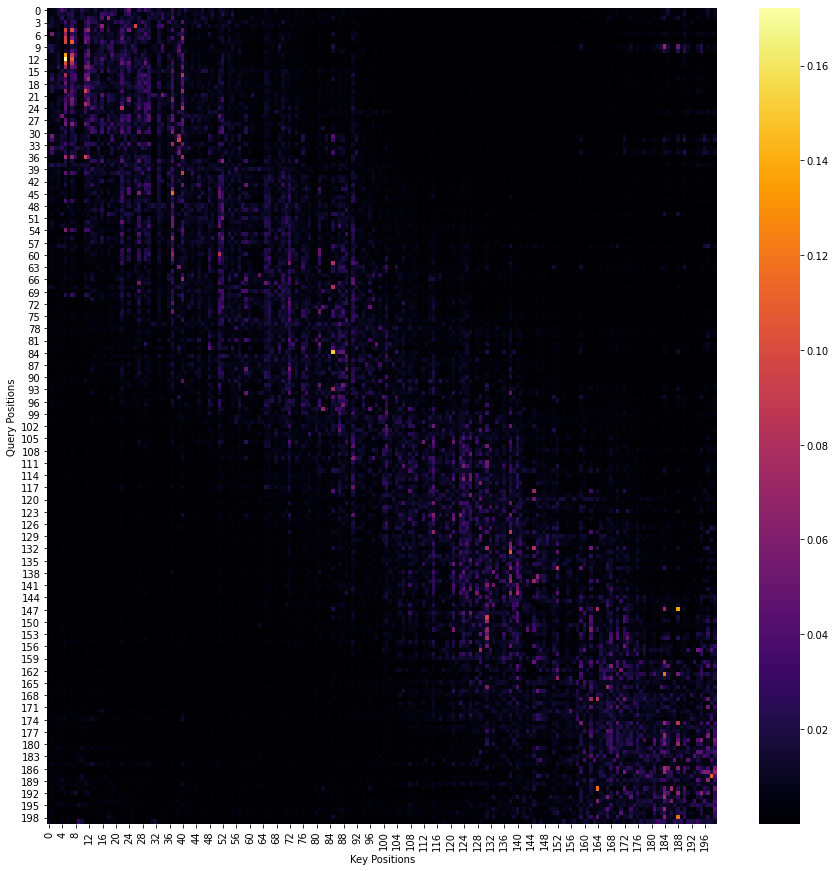
\includegraphics[width=.95\linewidth]{figures/attn1/L0BPH1.png}
    \caption{\textbf{Pos} Layer 0 Head 1}
  \end{subfigure}
  \begin{subfigure}[ht]{.33\linewidth}
    \centering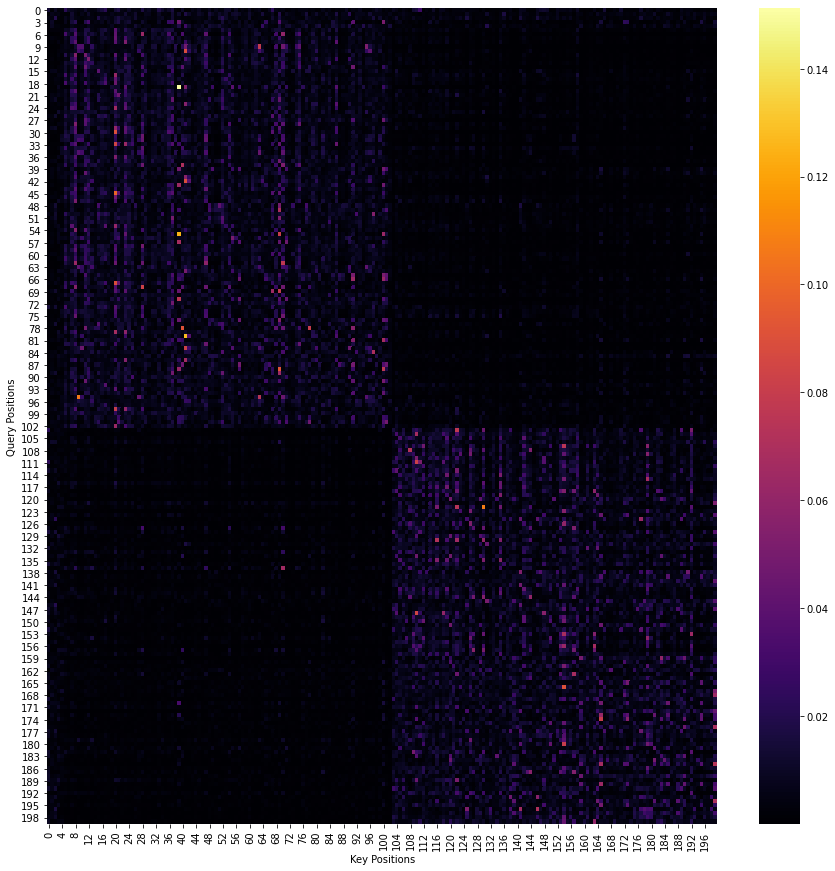
\includegraphics[width=.95\linewidth]{figures/attn1/L0BDH0.png}
    \caption{\textbf{Day} Layer 0 Head 0}
  \end{subfigure}
  \begin{subfigure}[ht]{.33\linewidth}
    \centering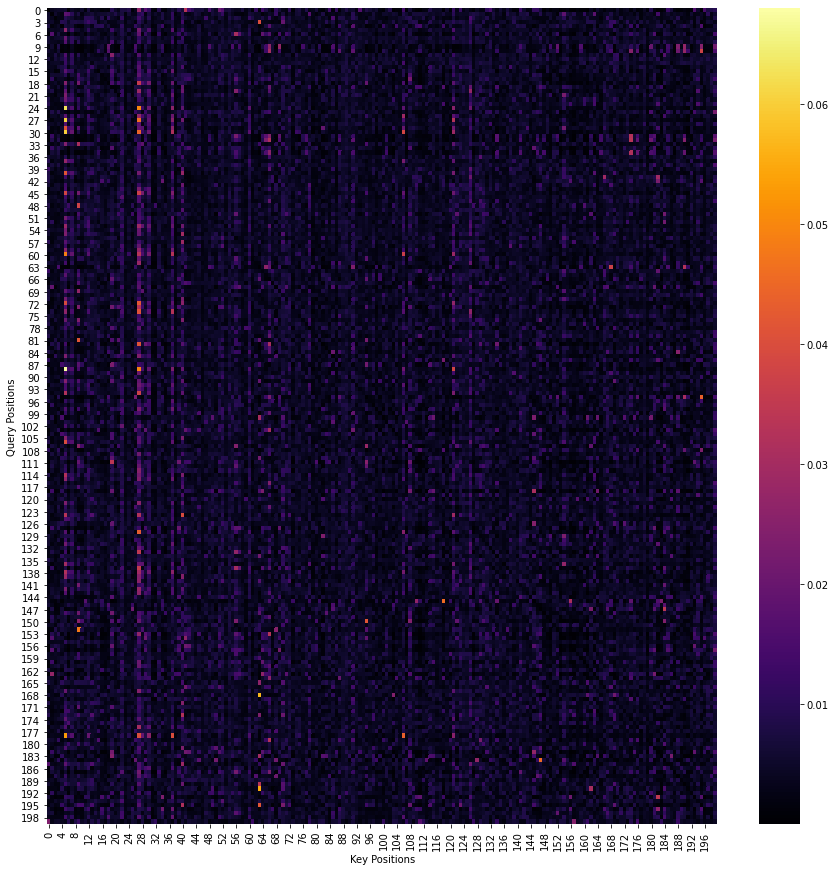
\includegraphics[width=.95\linewidth]{figures/attn1/L0BCH0.png}
    \caption{\textbf{Const} Layer 0 Head 0}
  \end{subfigure}
  \begin{subfigure}[ht]{.33\linewidth}
    \centering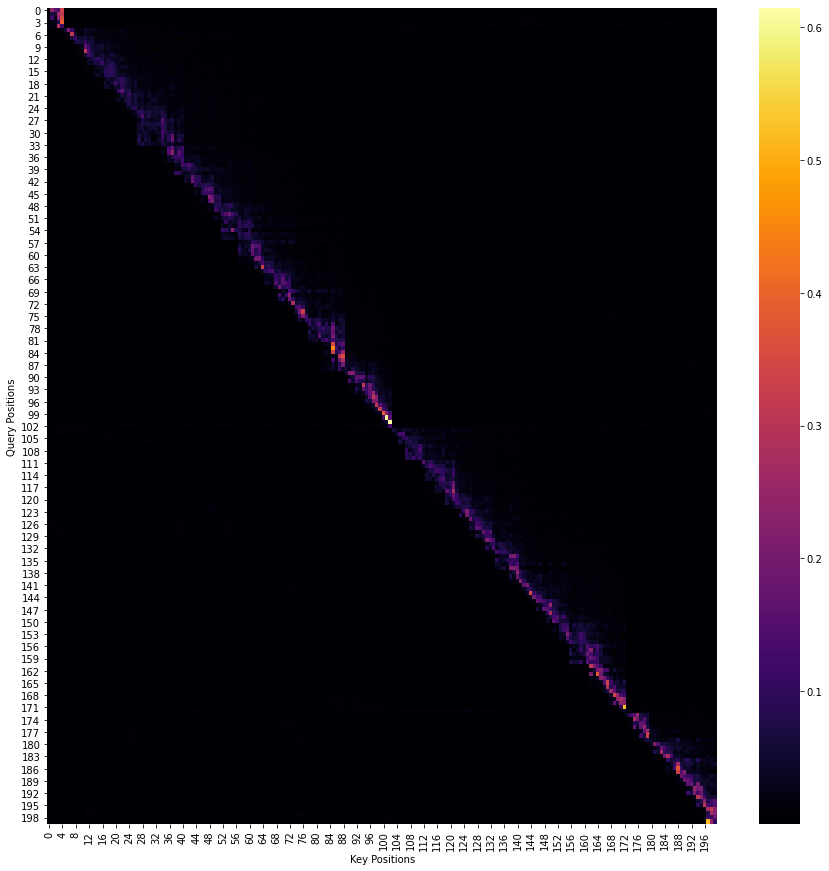
\includegraphics[width=.95\linewidth]{figures/attn1/L0BSH0.png}
    \caption{\textbf{Sinusoid} Layer 0 Head 0}
  \end{subfigure}
  \begin{subfigure}[ht]{.33\linewidth}
    \centering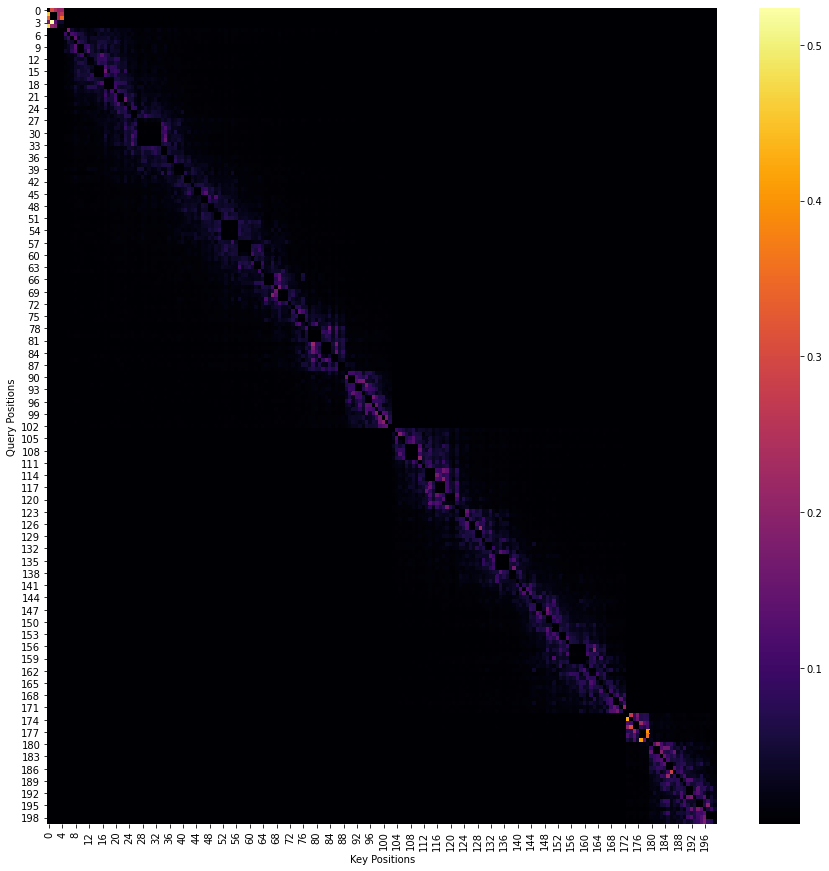
\includegraphics[width=.95\linewidth]{figures/attn1/L0BEH0.png}
    \caption{\textbf{Exp} Layer 0 Head 0}
  \end{subfigure}
  \begin{subfigure}[ht]{.33\linewidth}
    \centering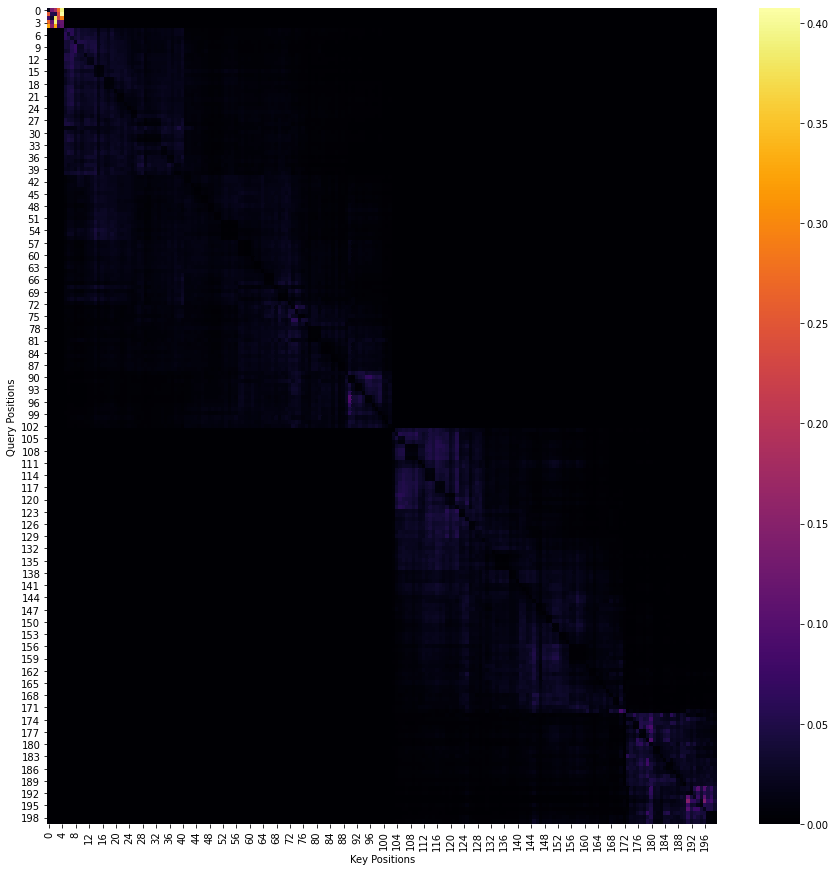
\includegraphics[width=.95\linewidth]{figures/attn1/L1BLH0.png}
    \caption{\textbf{Log1p} Layer 1 Head 0}
  \end{subfigure}
  
  %\subfigure{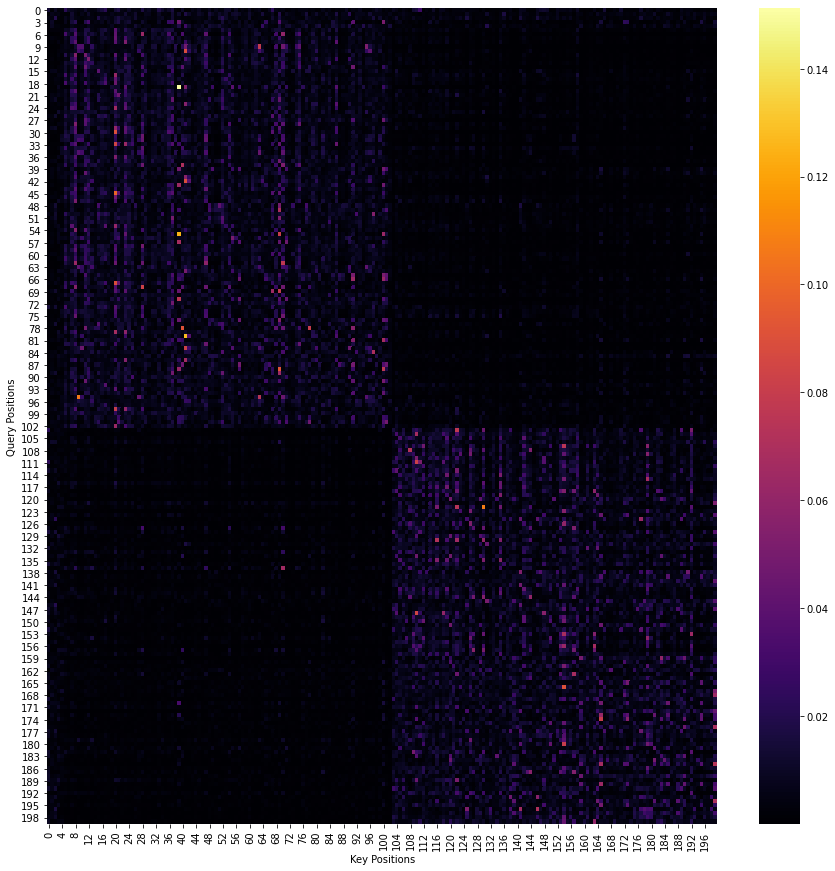
\includegraphics[width=0.5\linewidth]{figures/attn1/L0BDH0.png}}
  %\subfigure{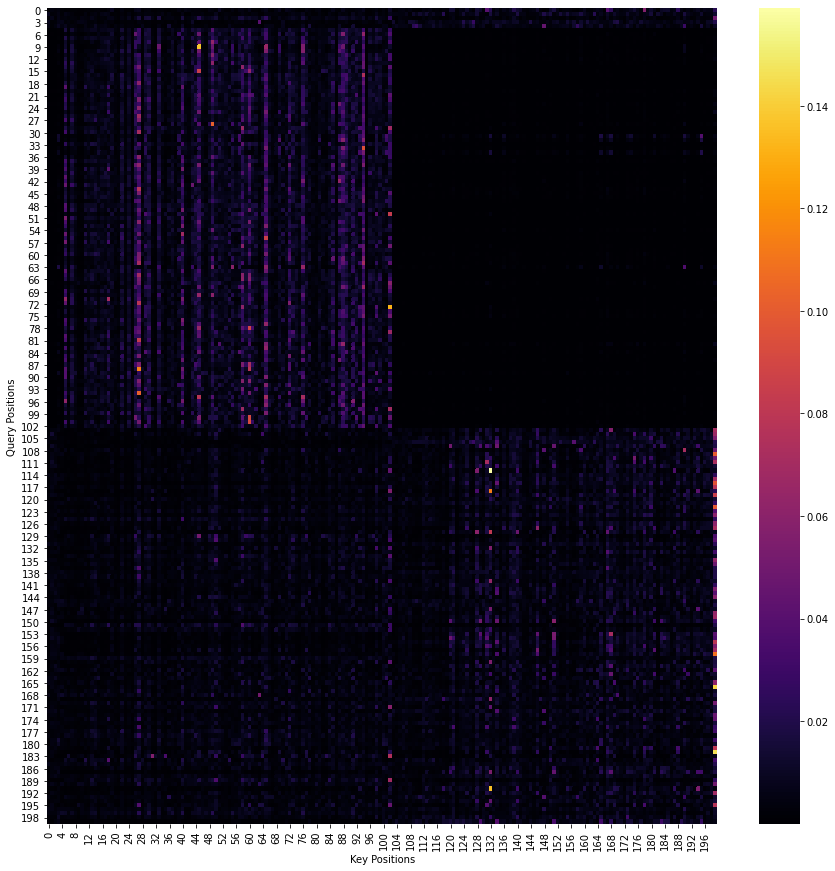
\includegraphics[width=0.5\linewidth]{figures/attn1/L0BDH1.png}}
  \caption{Attention Score Maps (Might need to change the figures to ones with shorter sequences (so that they are more clear))}
  \Description{TODO:Description}
  \label{fig:attnmaps}
\end{figure}
